% =========================================================================== %
% Yes. This is a document.

\documentclass[
	ngerman,
	aspectratio=169,
	table
]{beamer}

% =========================================================================== %
% Theme
\usepackage{scrlfile}
	\ReplacePackage{beamerthemeSHUR}{./sty/beamerthemeSHUR}
	\ReplacePackage{beamerinnerthemefancy}{./sty/beamerinnerthemefancy}
	\ReplacePackage{beamerouterthemedecolines}{./sty/beamerouterthemedecolines}
	\ReplacePackage{beamercolorthemechameleon}{./sty/beamercolorthemechameleon}

\usetheme[
	pageofpages=von,
	bullet=circle,
	titleline=true,
	alternativetitlepage=true,
	watermark="",
	watermarkheight=0px,
	watermarkheightmult=0
	]
{SHUR}

% =================================================================================================== %
% the usual stuff

\usepackage[utf8]{inputenc}
\usepackage[T1]{fontenc}
\usepackage{babel}
\usepackage{lmodern}
\usepackage{microtype}
\usepackage{csquotes}

\usepackage{tabularx}
\usepackage{booktabs}
\usepackage{multirow}

\usepackage{color, colortbl}
\usepackage{xcolor}

\usepackage{tabto}

\usepackage{minted}
	\usemintedstyle{friendly}

\usepackage{tikz}
	\usetikzlibrary{positioning}
	\usetikzlibrary{matrix}
	\usetikzlibrary{shapes.geometric}
	\usetikzlibrary{backgrounds}
	\usetikzlibrary{calc}
	\usetikzlibrary{decorations.pathreplacing}
	\tikzstyle{every picture}+=[remember picture] 
\usepackage{adjustbox}

\usepackage[most]{tcolorbox}
	\tcbsetforeverylayer
		{colback=cyan!10!white,
		 colframe=cyan!75!black,
		 arc=0pt,
		 outer arc=0pt
		}
	\newtcolorbox{codebox}[1][Code]
		{colback=black!5!white,
		 colframe=blue!40!black,
		 title=#1,
		 leftupper=6mm
		}
	\newtcolorbox{cmdbox}[1][Kommandozeilen-Befehl]
		{colback=black,
		 coltext=white,
		 fontupper=\ttfamily ,
		 colframe=blue!40!black,
		 title=#1,
		 outer arc=0pt
		}
	\newtcolorbox{warnbox}[1][Beachte]
		{colback=black!5!white,
		 colframe=red!40!black,
		 title=#1
		}
	\newtcolorbox{hintbox}[1][Tipp]
		{colback=black!5!white,
		 colframe=green!40!black,
		 title=#1
		}%
	\newenvironment{itembox}[1][]
		{\begin{tcolorbox}[title=#1]\begin{itemize}}%
		{\end{itemize}\end{tcolorbox}}
	\newtcolorbox{doublebox}[1][.3]
		{righthand width=#1\linewidth,
		 sidebyside,
		 sidebyside gap=6mm,
		 sidebyside align=center,
		 lower separated=false}

%==============================================================================%
% GLOBAL MACROS

\newcommand*{\zB}{z.\,B. }
\newcommand*{\ua}{u.\,a. }
\newcommand*{\ie}{d.\,h. }			%% dh is already a defined macro. Couldn't find out what it does.
\newcommand*{\idR}{i.\,d.\,R. }

\newcommand*{\tabcrlf}{\\ \midrule}			% actually still allows for optional argument

% =========================================================================== %

\author{Stefan Hartinger}
\title{Programmieren in C und C++}
\subtitle{Kursteil 7: Dynamische Speicherverwaltung}
\institute{Universität Regensburg, Fakultät Physik}
\date{Wintersemester 2020/21}

% =========================================================================== %

\begin{document}
% =========================================================================== %

\begin{frame}[t,plain]
\titlepage
\end{frame}

% =========================================================================== %

\begin{frame}{Recap}
%
Letzte Stunde haben wir gesehen/kennengelernt:
%
\begin{columns}[T]
\column{.5\linewidth}
\begin{itemize}
\item Konzept String: \mintinline{c}{char}-Array
\item Funktionen aus \emph{stringh.h}
	\begin{itemize}
	\item \texttt{strlen} -- Länge bestimmen
	\item \texttt{strcmp} -- Vergleichen
	\item \texttt{strcat} -- Verketten
	\item \texttt{strcpy} -- Kopieren
	\item \texttt{strchr} und \texttt{strrchr} -- Durchsuchen
	\item Varianten \texttt{memXXX} -- für allgemeine Arrays
	\end{itemize}
\end{itemize}
%
\column{.5\linewidth}
\begin{itemize}
\item \texttt{sprintf} -- formatierten String erstellen
\item Funktionenen in \texttt{ctype.h}
	\begin{itemize}
	\item \texttt{toupper} und \texttt{tolower}
	\item \texttt{isXXX}-Funktionen
	\end{itemize}
\item Funktionen in \texttt{stdlib.h}
	\begin{itemize}
	\item \texttt{atoXXX}-Funktionen
	\item Zufallszahlen mit \texttt{rand}
	\end{itemize}
\end{itemize}
\end{columns}
\begin{center}
\emph{Fragen hierzu?}
\end{center}
%
\end{frame}

% =========================================================================== %

\begin{frame}[fragile]{Recap}
%
Letzte Stunde haben wir gesehen/kennengelernt:
%
\begin{columns}[T]
\column{.5\linewidth}
\begin{itemize}
\item Funktionen
	\begin{itemize}
	\item explizite/implizite Deklaration
	\item Parameterliste
	\item Wertrückgabe mit \mintinline{c}{return}
	\item Übergabe \enquote{byRef}: Als Pointer
	\item Datentyp \mintinline{c}{void}
	\end{itemize}
\end{itemize}
%
\column{.5\linewidth}
\begin{itemize}
\item Scopes
	\begin{itemize}
	\item Sichtbarkeit von Variablen
	\item \enquote{von außen nach innen}
	\item Keine \enquote{Quer-Sichtbarkeit}
	\item Globale Variablen
	\end{itemize}
\item \emph{Fragen hierzu?}
\end{itemize}
\end{columns}
%
\end{frame}

% =========================================================================== %

\begin{frame}[fragile]%{Aus den letzten Übungen}
%
\tcbset{width=.495\linewidth, height=7.8cm, on line}
%
\begin{codebox}[Aufgabe \enquote{Bubble Sort}]
\begin{minted}[fontsize=\scriptsize,linenos]{c}
#include <stdio.h>
#include <stdlib.h>
#include <time.h>

int main () {
  int Lo = 1, Hi = 100;
  int nums[1024];
  int N, i, dummy;
  int flagSwap = 0;
  int countSwaps = 0;

  printf("List item count?\n");
  scanf("%d", &N);
  srand(time(NULL));
  
  printf("Numbers, unsorted:\n");
  for (i=0; i<N; i++) {
    nums[i] = Lo + rand() % (Hi-Lo+1);
    printf("%d\n", numbers[i]);
  }
\end{minted}
\end{codebox}
%
\begin{codebox}[...Fortsetzung]
\begin{minted}[fontsize=\scriptsize, linenos, firstnumber=last]{c}
  do {
    flagSwap = 0;
    for (i = 0; i < N-1; i++) {
      if (nums[i] > nums[i+1]) {
        flagSwap = 1;
        countSwaps++;
	    
        dummy     = nums[i  ];
        nums[i  ] = nums[i+1];
        nums[i+1] = dummy;
      }
    }
  } while(flagSwap);

  printf("Sorted List (%d swaps):\n", 
    countSwaps);
  for (i=0; i<N; i++) {
    printf("%d\n", nums[i]);
  }
}
\end{minted}
\end{codebox}
%
\end{frame}

% =========================================================================== %

\begin{frame}[fragile]{Aus den letzten Übungen}
%
\tcbset{width=.52\linewidth, on line, height=6.3cm}
\begin{codebox}[Aufgabe: Swap]
\begin{minted}[fontsize=\scriptsize, linenos]{c}
#include <stdio.h>

void swapDoubles (double * x, double * y) {
  double dummy = *y;
  *y = *x;
  *x = dummy;
}

int main () {
  double a = 1.3;
  double b = 7.7;
  
  printf("a = %f\tb = %f\n", a, b);
  swapDoubles( &a, &b );
  printf("a = %f\tb = %f\n", a, b);
}
\end{minted}
\end{codebox}
%
\tcbset{width=.45\linewidth, on line, height=6.3cm}
\begin{tcolorbox}[title=Speicherbild, valign=center]
\renewcommand{\arraystretch}{1.5}
\tiny
\begin{tabular}{c|c|c|c|c|c|c}
\ldots &   x  &   y  & dummy & \ldots &  a  &  b  \\ \hline
\ldots & (??) & (??) &  (??) & \ldots & 1.3 & 7.7 \\
\multicolumn{7}{c}{$\Downarrow$}\\
\ldots & \&a  & \&b  &  (??) & \ldots & 1.3 & 7.7 \\
\multicolumn{7}{c}{$\Downarrow$}\\
\ldots & \&a  & \&b  &  7.7 & \ldots & 1.3 & 7.7 \\
\multicolumn{7}{c}{$\Downarrow$}\\
\ldots & \&a  & \&b  &  7.7 & \ldots & 1.3 & 1.3 \\
\multicolumn{7}{c}{$\Downarrow$}\\
\ldots & \&a  & \&b  &  7.7 & \ldots & 7.7 & 1.3 \\
\multicolumn{7}{c}{$\Downarrow$}\\
\ldots & (??) & (??) &  (??) & \ldots & 7.7 & 1.3 \\
\end{tabular}
\end{tcolorbox}
%
\end{frame}

% =========================================================================== %

\begin{frame}[fragile]{Aus der letzten Übung: Quersumme mit Strings}
%
\tcbset{width=.495\linewidth, on line, height=6.5cm}
\begin{codebox}[Quersumme mit Strings]
\begin{minted}[fontsize=\scriptsize, linenos]{c}
#include <stdio.h>

int crosssum(int number) {
   char snum[20] = {};
   int  reVal    =  0;

   sprintf(snum, "%d", number);
   for (int i=0; i<20; i++) {
      reVal += (
         (snum[i] >= '0') && 
         (snum[i] <= '9')
      ) ? snum[i] - '0' : 0;
   }

   return reVal;
}
\end{minted}
\end{codebox}
%
\begin{codebox}[...Fortsetzung]
\begin{minted}[fontsize=\scriptsize, linenos, firstnumber=last]{c}
int main (void) {
   int a = 0;

   printf("Please enter an integer: ");
   scanf("%d", &a);

   printf(
      "The cross sum of %d is %d.\n",
      a, crosssum(a)
   );
}
\end{minted}
\end{codebox}
%
\end{frame}

% =========================================================================== %

\begin{frame}[fragile]{Aus der letzten Übung: Quersumme ohne Strings}
%
\tcbset{width=.495\linewidth, on line, height=5cm}
\begin{codebox}[Quersumme ohne Strings]
\begin{minted}[fontsize=\scriptsize, linenos]{c}
#include <stdio.h>

int crosssum(int a) {
   int reVal = 0;

   do {
      reVal += a % 10;
      a /= 10;
   } while(a);

   return reVal;
}
\end{minted}
\end{codebox}
%
\begin{codebox}[...Fortsetzung]
\begin{minted}[fontsize=\scriptsize, linenos, firstnumber=last]{c}
int main (void) {
   int a;

   printf("please enter a number:\n");
   scanf("%d", &a);

   printf(
      "The cross sum of %d is %d.\n",
      a, crosssum(a)
   );
}
\end{minted}
\end{codebox}
%
%$\Rightarrow$ Schneller und weniger Fehleranfällig.
\tcbset{width=\linewidth, height=1.5cm}
\begin{hintbox}
Strings wo möglich vermeiden
\end{hintbox}
%
\end{frame}

% =========================================================================== %

\begin{frame}{Script}
%
\begin{itemize}
\item Kapitel 8
	\begin{itemize}
	\item 8.2. Dynamische Speicherverwaltung
		\begin{itemize}
		\item 8.2.1. Speicher allozieren und freigeben: \texttt{malloc}, \texttt{calloc} und \texttt{free}
		\item 8.2.2. Feldgrößen ändern: \texttt{realloc}
		\item 8.2.3. Heap und Stack
		\item 8.2.5. mehrdimensionale dynamische Arrays
		\end{itemize}
	\end{itemize}
\end{itemize}
%
\end{frame}

% =========================================================================== %

\begin{frame}[fragile]{Wiederholung -- Scopes und \enquote{Lebensdauer} von Variablen}
%
\begin{columns}[T]
\column{.5\linewidth}
\begin{itemize}
\item Variablen existieren nur innerhalb  ihres Scopes
\item Wird Scope verlassen, so wird auch der Speicherbereich der Variablne frei gegeben
\item Pointer können weiter darauf verweisen, sind dann aber ungültig
\item Lösung: Variablen im \enquote{richtigen} Scope anlegen -- notfalls: Global
\item Function \texttt{prepArray} nur zum Befüllen nutzen
\item Oder: Dynamische Speicherverwaltung
\end{itemize}
%
\column{.5\linewidth}
\begin{warnbox}[Arrayzugriff außerhalb Lebensdauer, leftupper=6mm]
\begin{minted}[fontsize=\scriptsize, linenos]{c}
#include <stdio.h>

int * prepArray() {
  int array[] = {1, 2, 3};
  return array;
}

int main () {
  int * array = prepArray();
  
  // Programm könnte hier abstürzen
  array[1] = 7;
}
\end{minted}
\end{warnbox}
\end{columns}
%
\end{frame}

% =========================================================================== %

\begin{frame}[fragile]
%
\begin{columns}[T]
\column{.48\linewidth}
\begin{Large}
Dynamische Speicherverwaltung: Ausgangsproblem
\vspace{10pt}
\end{Large}
%
\begin{itemize}
\item Unterscheidung: \emph{Kompilierzeit} und \emph{Laufzeit}
	\begin{itemize}
	\item Kompilierzeit: Wenn das Programm geschrieben wird
	\item Laufzeit: Wenn es ausgeführt wird.
	\end{itemize}
\item Zur Kompilierzeit: Nicht alle Informationen verfügbar!
\item Beispiel: Wie viele Datensätze verarbeiten?
\item Code muss daher \emph{allgemeingültig} geschrieben werden.
\item Bisher: \enquote{Puffer}-Lösungen
\end{itemize}
%
\column{.53\linewidth}
\begin{codebox}[Beispiel: Liste von Zufallszahlen, height=7.7cm]
\begin{minted}[fontsize=\scriptsize, linenos]{c}
#include <stdio.h>
#include <stdlib.h>
#include <time.h>

int main () {
  int i, N, numbers[1024];
  
  printf("generate how many numbers?\n");
  scanf("%d", &N);
  if (N > 1024) {
    printf("not enough memory!\n");
    return -1; // for OS: process failed
  }
  
  srand(time(NULL));
  for (i=0; i<N; i++) {
    numbers[i] = rand();
  }
  return 0; // for OS: everything all right
}
\end{minted}
\end{codebox}
\end{columns}

%
\end{frame}

% =========================================================================== %

\begin{frame}[fragile]{Dynamische Speicherverwaltung: Memory Allocation}
%
\begin{columns}[T]
\column{.5\linewidth}
\begin{itemize}
\item Aus \texttt{stdlib.h}: Befehl \texttt{malloc}
	\begin{itemize}
	\item Reserviert $N$ zusammenhängende Bytes im Speicher
	\item Gibt Pointer auf Anfang des reservierten Bereichs zurück
	\item Gibt bei Fehler \texttt{NULL} zurück
	\end{itemize}
\item Speicher muss nach Verwendung frei gegeben werden
\begin{itemize}
	\item \texttt{free} aus \texttt{stdlib.h}
	\item Darf nur auf \emph{dynamische Pointer} angewandt werden
	\item Darf auf einen Pointer \emph{genau ein mal} angewandt werden.
	\item Darf nicht auf \texttt{NULL} angewandt werden
\end{itemize}

\end{itemize}
%
\column{.5\linewidth}
\begin{codebox}[Syntax: malloc]
\begin{minted}[fontsize=\scriptsize]{c}
Datentyp * var = malloc(N);
\end{minted}
\end{codebox}
%
\begin{codebox}[Syntax: free]
\begin{minted}[fontsize=\scriptsize]{c}
free(var);
\end{minted}
\end{codebox}
%
\begin{hintbox}
Beim Tippen von \texttt{malloc} sofort das zugehörige \texttt{free} schreiben -- erst dann den Code, der das Array benutzt
\end{hintbox}
\end{columns}

%
\end{frame}

% =========================================================================== %

\begin{frame}[fragile]
%

\begin{codebox}[Beispiel: Zufallszahlen mit dynamischen Arrays]
\begin{minted}[fontsize=\scriptsize, linenos]{c}
#include <stdio.h>
#include <stdlib.h>
#include <time.h>

int main () {
  int i, N; srand(time(NULL));
  printf("generate how many numbers?\n"); scanf("%d", &N);
  
  int * willy = malloc(N * sizeof(int));
  if (!willy) {
    printf("failed to allocate memory!\n");
    return -1;	// for OS: process failed
  }
  
  for (i=0; i<N; i++) {willy[i] = rand();}
  for (i=0; i<N; i++) {printf("%d\n", willy[i]);}
  
  free(willy);
  return 0; // for OS: everything all right
}
\end{minted}
\end{codebox}
%
\end{frame}

% =========================================================================== %

\begin{frame}[fragile]
%
\begin{columns}[T]
\column{.5\linewidth}
\begin{Large}
Pointer beliebigen Typs -- \mintinline{c}{void *}
\end{Large}
%
\begin{itemize}
\item \texttt{malloc} und \texttt{free} \enquote{wissen nicht}, welchen Pointer-Typ sie zurück geben sollen.
\item \mintinline{c}{void *} -- allgemeiner Pointer
\item Warnung, wenn Zuweisung von/zu Nicht-Pointer-Typen
\item Keine Dereferenzierung, kein Index-Zugriff
\item Pointer-Arithmetik: Wie \mintinline{c}{char}
\item So auch bei \texttt{memcpy}, \ldots
\end{itemize}
%
\column{.5\linewidth}
\begin{codebox}[Beispiel: Keine Prüfung des Datentyps]
\begin{minted}[fontsize=\scriptsize, linenos]{c}
int     * x = malloc(sizeof(int));
double  * y = malloc(sizeof(double));

// warning -- incompatible types
double  * z = x;

// invalid -- pointer to scalar
// double d = x;

// valid statement, no warning
void    * v = x;

// invalid use of void object
// printf("%lf\n", *v);  // x

free(x);
free(y);
// free(z) -- error -- already free'd
\end{minted}
\end{codebox}
\end{columns}

%
\end{frame}

% =========================================================================== %

\begin{frame}[fragile]{\texttt{calloc} und \texttt{realloc}}
%
\tcbset{width=.495\linewidth, on line, height=4.3cm}
%
\begin{itembox}[\texttt{calloc}]
\item wie \texttt{malloc}, aber setzt alle Bytes auf \mintinline{c}{0}
\item \enquote{allocate and clear}
\item langsamer, aber geringere Fehler-Gefahr
\item Syntax \emph{fast} identisch
\end{itembox}
%
\begin{itembox}[\texttt{realloc}]
\item \emph{redimensioniert} bestehendes Array
\item Bereits gespeicherte Werte bleiben erhalten.
\item Kann Werte \enquote{umziehen lassen}
\item Arraygröße \mintinline{c}{0} nicht zulässig
\end{itembox}
%
\tcbset{width=.495\linewidth, on line, height=1.5cm}
%
\begin{codebox}[Syntax]
\begin{minted}[fontsize=\scriptsize]{c}
ptr = calloc(itemCount, itemSizeBytes)
\end{minted}
\end{codebox}
%
\begin{codebox}[Syntax]
\begin{minted}[fontsize=\scriptsize]{c}
ptr = realloc(ptr, newSizeBytes)
\end{minted}
\end{codebox}
%
\end{frame}

% =========================================================================== %

\begin{frame}{Zum Syntax-Unterschied \texttt{malloc} vs. \texttt{calloc}}
%
\begin{columns}
\column{.5\linewidth}
\begin{center}

\includegraphics[width=\linewidth]{./gfx/xkcd_standards}
\newline
\tiny\url{https://xkcd.com/927/}
\end{center}
%
\column{.5\linewidth}
\begin{hintbox}
Macht euch vor Projektbeginn Gedanken über einheitliche Logik! (Parameter-Reihenfolge, Variablen-Benennung, Code-Struktur, \ldots)
\end{hintbox}
%
\begin{hintbox}
Im Zweifel könnt ihr immer in der CPP-Referenz nachschlagen!
\end{hintbox}
\end{columns}
%
\end{frame}

% =========================================================================== %

\begin{frame}{Speicherbild: Vergrößerung (I)}
%
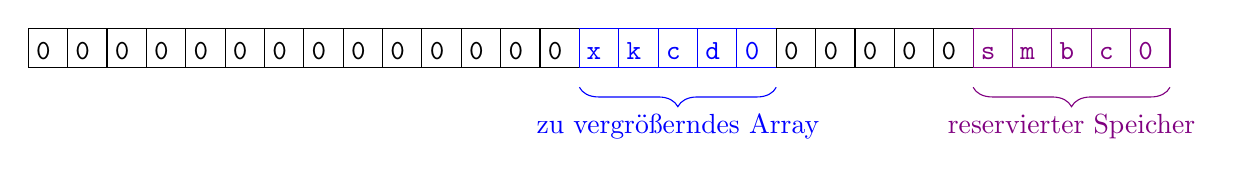
\begin{tikzpicture}
  [ 
    cell/.style={
       text width =3mm,
       text height=3mm, 
       draw=black, 
       inner sep=1mm
    },
    ld/.style={
       draw=blue,
       shorten >=2pt,
       ->
    }
  ]
  \node (c00) at ( 0.0,1) [cell]         {\ttfamily 0};
  \node (c01) at ( 0.5,1) [cell]         {\ttfamily 0};
  \node (c02) at ( 1.0,1) [cell]         {\ttfamily 0};
  \node (c03) at ( 1.5,1) [cell]         {\ttfamily 0};
  \node (c04) at ( 2.0,1) [cell]         {\ttfamily 0};
  \node (c05) at ( 2.5,1) [cell]         {\ttfamily 0};
  \node (c06) at ( 3.0,1) [cell]         {\ttfamily 0};
  \node (c07) at ( 3.5,1) [cell]         {\ttfamily 0};
  \node (c08) at ( 4.0,1) [cell]         {\ttfamily 0};
  \node (c09) at ( 4.5,1) [cell]         {\ttfamily 0};
  \node (c10) at ( 5.0,1) [cell]         {\ttfamily 0};
  \node (c11) at ( 5.5,1) [cell]         {\ttfamily 0};
  \node (c12) at ( 6.0,1) [cell]         {\ttfamily 0};
  \node (c13) at ( 6.5,1) [cell]         {\ttfamily 0};
  \node (c14) at ( 7.0,1) [cell, blue]   {\ttfamily x};
  \node (c15) at ( 7.5,1) [cell, blue]   {\ttfamily k};
  \node (c16) at ( 8.0,1) [cell, blue]   {\ttfamily c};
  \node (c17) at ( 8.5,1) [cell, blue]   {\ttfamily d};
  \node (c18) at ( 9.0,1) [cell, blue]   {\ttfamily 0};
  \node (c19) at ( 9.5,1) [cell]         {\ttfamily 0};
  \node (c20) at (10.0,1) [cell]         {\ttfamily 0};
  \node (c21) at (10.5,1) [cell]         {\ttfamily 0};
  \node (c22) at (11.0,1) [cell]         {\ttfamily 0};
  \node (c23) at (11.5,1) [cell]         {\ttfamily 0};
  \node (c24) at (12.0,1) [cell, violet] {\ttfamily s};
  \node (c25) at (12.5,1) [cell, violet] {\ttfamily m};
  \node (c26) at (13.0,1) [cell, violet] {\ttfamily b};
  \node (c27) at (13.5,1) [cell, violet] {\ttfamily c};
  \node (c28) at (14.0,1) [cell, violet] {\ttfamily 0};
  
  \draw [decorate, decoration={brace,amplitude=7pt, mirror}, xshift=-0pt, yshift=0pt, blue]
  		( 6.75, 0.5) -- ( 9.25, 0.5) node [blue, midway, yshift=-0.5cm] 
		(braceArrayPreResize) {zu vergrößerndes Array};

  \draw [decorate, decoration={brace,amplitude=7pt, mirror}, xshift=-0pt, yshift=0pt, violet]
  		(11.75, 0.5) -- (14.25, 0.5) node [violet, midway, yshift=-0.5cm] 
		(braceArrayPreResize) {reservierter Speicher};
\end{tikzpicture}
%
%
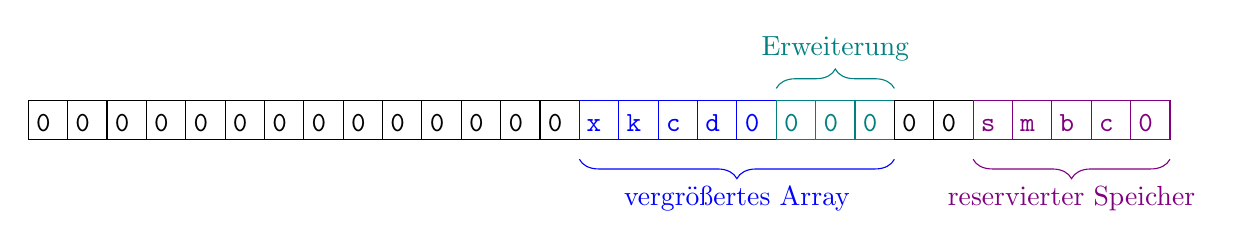
\begin{tikzpicture}
  [ 
    cell/.style={
       text width =3mm,
       text height=3mm, 
       draw=black, 
       inner sep=1mm
    },
    ld/.style={
       draw=blue,
       shorten >=2pt,
       ->
    }
  ]
  \node (c00) at ( 0.0,1) [cell]         {\ttfamily 0};
  \node (c01) at ( 0.5,1) [cell]         {\ttfamily 0};
  \node (c02) at ( 1.0,1) [cell]         {\ttfamily 0};
  \node (c03) at ( 1.5,1) [cell]         {\ttfamily 0};
  \node (c04) at ( 2.0,1) [cell]         {\ttfamily 0};
  \node (c05) at ( 2.5,1) [cell]         {\ttfamily 0};
  \node (c06) at ( 3.0,1) [cell]         {\ttfamily 0};
  \node (c07) at ( 3.5,1) [cell]         {\ttfamily 0};
  \node (c08) at ( 4.0,1) [cell]         {\ttfamily 0};
  \node (c09) at ( 4.5,1) [cell]         {\ttfamily 0};
  \node (c10) at ( 5.0,1) [cell]         {\ttfamily 0};
  \node (c11) at ( 5.5,1) [cell]         {\ttfamily 0};
  \node (c12) at ( 6.0,1) [cell]         {\ttfamily 0};
  \node (c13) at ( 6.5,1) [cell]         {\ttfamily 0};
  \node (c14) at ( 7.0,1) [cell, blue]   {\ttfamily x};
  \node (c15) at ( 7.5,1) [cell, blue]   {\ttfamily k};
  \node (c16) at ( 8.0,1) [cell, blue]   {\ttfamily c};
  \node (c17) at ( 8.5,1) [cell, blue]   {\ttfamily d};
  \node (c18) at ( 9.0,1) [cell, blue]   {\ttfamily 0};
  \node (c19) at ( 9.5,1) [cell, teal]   {\ttfamily 0};
  \node (c20) at (10.0,1) [cell, teal]   {\ttfamily 0};
  \node (c21) at (10.5,1) [cell, teal]   {\ttfamily 0};
  \node (c22) at (11.0,1) [cell]         {\ttfamily 0};
  \node (c23) at (11.5,1) [cell]         {\ttfamily 0};
  \node (c24) at (12.0,1) [cell, violet] {\ttfamily s};
  \node (c25) at (12.5,1) [cell, violet] {\ttfamily m};
  \node (c26) at (13.0,1) [cell, violet] {\ttfamily b};
  \node (c27) at (13.5,1) [cell, violet] {\ttfamily c};
  \node (c28) at (14.0,1) [cell, violet] {\ttfamily 0};
  
  \draw [decorate, decoration={brace,amplitude=7pt, mirror}, xshift=-0pt, yshift=0pt, blue]
  		( 6.75, 0.5) -- (10.75, 0.5) node [blue, midway, yshift=-0.5cm] 
		(braceArrayPreResize) {vergrößertes Array};

  \draw [decorate, decoration={brace,amplitude=7pt, mirror}, xshift=-0pt, yshift=0pt, violet]
  		(11.75, 0.5) -- (14.25, 0.5) node [violet, midway, yshift=-0.5cm] 
		(braceArrayPreResize) {reservierter Speicher};

  \draw [decorate, decoration={brace,amplitude=7pt}, xshift=-0pt, yshift=0pt, teal]
  		( 9.25, 1.4) -- (10.75, 1.4) node [teal, midway, yshift=+0.5cm] 
		(braceArrayPreResize) {Erweiterung};
\end{tikzpicture}
%
\end{frame}

% =========================================================================== %

\begin{frame}{Speicherbild: Vergrößerung (II)}
%
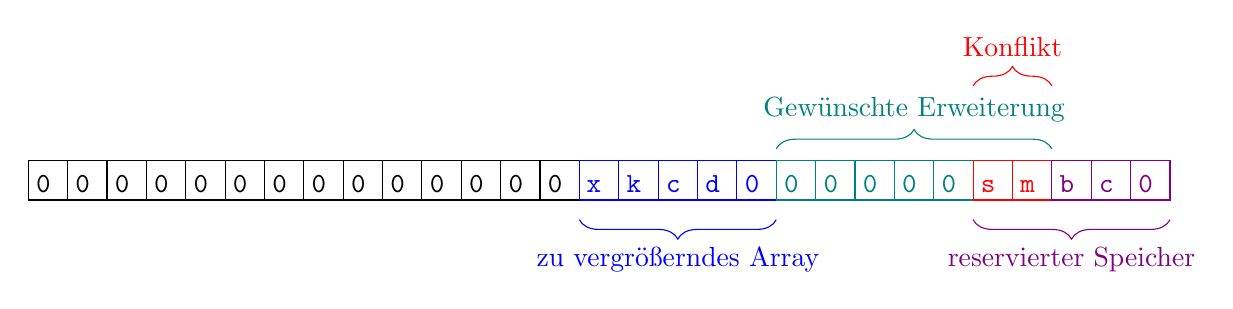
\begin{tikzpicture}
  [ 
    cell/.style={
       text width =3mm,
       text height=3mm, 
       draw=black, 
       inner sep=1mm
    },
    ld/.style={
       draw=blue,
       shorten >=2pt,
       ->
    }
  ]
  \node (c00) at ( 0.0,1) [cell]         {\ttfamily 0};
  \node (c01) at ( 0.5,1) [cell]         {\ttfamily 0};
  \node (c02) at ( 1.0,1) [cell]         {\ttfamily 0};
  \node (c03) at ( 1.5,1) [cell]         {\ttfamily 0};
  \node (c04) at ( 2.0,1) [cell]         {\ttfamily 0};
  \node (c05) at ( 2.5,1) [cell]         {\ttfamily 0};
  \node (c06) at ( 3.0,1) [cell]         {\ttfamily 0};
  \node (c07) at ( 3.5,1) [cell]         {\ttfamily 0};
  \node (c08) at ( 4.0,1) [cell]         {\ttfamily 0};
  \node (c09) at ( 4.5,1) [cell]         {\ttfamily 0};
  \node (c10) at ( 5.0,1) [cell]         {\ttfamily 0};
  \node (c11) at ( 5.5,1) [cell]         {\ttfamily 0};
  \node (c12) at ( 6.0,1) [cell]         {\ttfamily 0};
  \node (c13) at ( 6.5,1) [cell]         {\ttfamily 0};
  \node (c14) at ( 7.0,1) [cell, blue]   {\ttfamily x};
  \node (c15) at ( 7.5,1) [cell, blue]   {\ttfamily k};
  \node (c16) at ( 8.0,1) [cell, blue]   {\ttfamily c};
  \node (c17) at ( 8.5,1) [cell, blue]   {\ttfamily d};
  \node (c18) at ( 9.0,1) [cell, blue]   {\ttfamily 0};
  \node (c19) at ( 9.5,1) [cell, teal]   {\ttfamily 0};
  \node (c20) at (10.0,1) [cell, teal]   {\ttfamily 0};
  \node (c21) at (10.5,1) [cell, teal]   {\ttfamily 0};
  \node (c22) at (11.0,1) [cell, teal]   {\ttfamily 0};
  \node (c23) at (11.5,1) [cell, teal]   {\ttfamily 0};
  \node (c24) at (12.0,1) [cell, red]    {\ttfamily s};
  \node (c25) at (12.5,1) [cell, red]    {\ttfamily m};
  \node (c26) at (13.0,1) [cell, violet] {\ttfamily b};
  \node (c27) at (13.5,1) [cell, violet] {\ttfamily c};
  \node (c28) at (14.0,1) [cell, violet] {\ttfamily 0};
  
  \draw [decorate, decoration={brace,amplitude=7pt, mirror}, xshift=-0pt, yshift=0pt, blue]
  		( 6.75, 0.5) -- ( 9.25, 0.5) node [blue, midway, yshift=-0.5cm] 
		(braceArrayPreResize) {zu vergrößerndes Array};

  \draw [decorate, decoration={brace,amplitude=7pt, mirror}, xshift=-0pt, yshift=0pt, violet]
  		(11.75, 0.5) -- (14.25, 0.5) node [violet, midway, yshift=-0.5cm] 
		(braceArrayPreResize) {reservierter Speicher};

  \draw [decorate, decoration={brace,amplitude=7pt}, xshift=-0pt, yshift=0pt, teal]
  		( 9.25, 1.4) -- (12.75, 1.4) node [teal, midway, yshift=+0.5cm] 
		(braceArrayPreResize) {Gewünschte Erweiterung};

  \draw [decorate, decoration={brace,amplitude=7pt}, xshift=-0pt, yshift=0pt, red]
  		(11.75, 2.2) -- (12.75, 2.2) node [red, midway, yshift=+0.5cm] 
		(braceArrayPreResize) {Konflikt};
\end{tikzpicture}
%
%
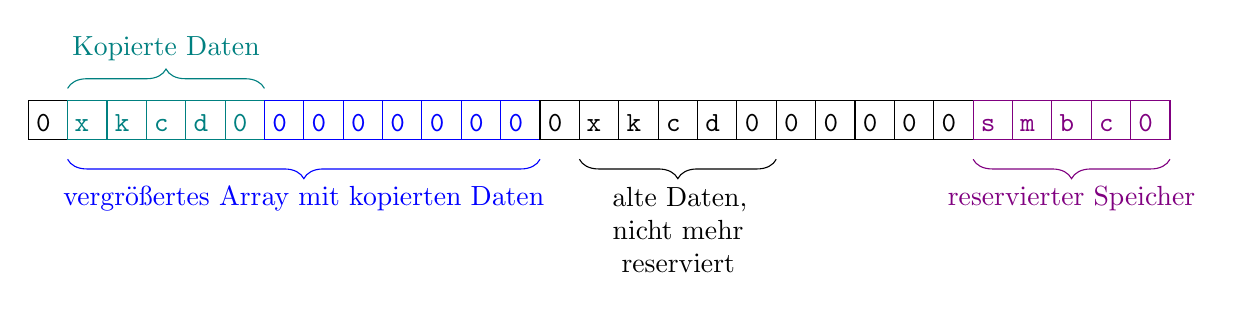
\begin{tikzpicture}
  [ 
    cell/.style={
       text width =3mm,
       text height=3mm, 
       draw=black, 
       inner sep=1mm
    },
    ld/.style={
       draw=blue,
       shorten >=2pt,
       ->
    }
  ]
  \node (c00) at ( 0.0,1) [cell]         {\ttfamily 0};
  \node (c01) at ( 0.5,1) [cell, teal]   {\ttfamily x};
  \node (c02) at ( 1.0,1) [cell, teal]   {\ttfamily k};
  \node (c03) at ( 1.5,1) [cell, teal]   {\ttfamily c};
  \node (c04) at ( 2.0,1) [cell, teal]   {\ttfamily d};
  \node (c05) at ( 2.5,1) [cell, teal]   {\ttfamily 0};
  \node (c06) at ( 3.0,1) [cell, blue]   {\ttfamily 0};
  \node (c07) at ( 3.5,1) [cell, blue]   {\ttfamily 0};
  \node (c08) at ( 4.0,1) [cell, blue]   {\ttfamily 0};
  \node (c09) at ( 4.5,1) [cell, blue]   {\ttfamily 0};
  \node (c10) at ( 5.0,1) [cell, blue]   {\ttfamily 0};
  \node (c11) at ( 5.5,1) [cell, blue]   {\ttfamily 0};
  \node (c12) at ( 6.0,1) [cell, blue]   {\ttfamily 0};
  \node (c13) at ( 6.5,1) [cell]         {\ttfamily 0};
  \node (c14) at ( 7.0,1) [cell]         {\ttfamily x};
  \node (c15) at ( 7.5,1) [cell]         {\ttfamily k};
  \node (c16) at ( 8.0,1) [cell]         {\ttfamily c};
  \node (c17) at ( 8.5,1) [cell]         {\ttfamily d};
  \node (c18) at ( 9.0,1) [cell]         {\ttfamily 0};
  \node (c19) at ( 9.5,1) [cell]         {\ttfamily 0};
  \node (c20) at (10.0,1) [cell]         {\ttfamily 0};
  \node (c21) at (10.5,1) [cell]         {\ttfamily 0};
  \node (c22) at (11.0,1) [cell]         {\ttfamily 0};
  \node (c23) at (11.5,1) [cell]         {\ttfamily 0};
  \node (c24) at (12.0,1) [cell, violet] {\ttfamily s};
  \node (c25) at (12.5,1) [cell, violet] {\ttfamily m};
  \node (c26) at (13.0,1) [cell, violet] {\ttfamily b};
  \node (c27) at (13.5,1) [cell, violet] {\ttfamily c};
  \node (c28) at (14.0,1) [cell, violet] {\ttfamily 0};
  
  \draw [decorate, decoration={brace,amplitude=7pt, mirror}, xshift=-0pt, yshift=0pt, blue]
  		( 0.25, 0.5) -- ( 6.25, 0.5) node [blue, midway, yshift=-0.5cm] 
		(braceArrayPreResize) {vergrößertes Array mit kopierten Daten};

  \draw [decorate, decoration={brace,amplitude=7pt, mirror}, xshift=-0pt, yshift=0pt, violet]
  		(11.75, 0.5) -- (14.25, 0.5) node [violet, midway, yshift=-0.5cm] 
		(braceArrayPreResize) {reservierter Speicher};

  \draw [decorate, decoration={brace,amplitude=7pt}, xshift=-0pt, yshift=0pt, teal]
  		( 0.25, 1.4) -- ( 2.75, 1.4) node [teal, midway, yshift=+0.5cm] 
		(braceArrayPreResize) {Kopierte Daten};
  
  \draw [decorate, decoration={brace,amplitude=7pt, mirror}, xshift=-0pt, yshift=0pt, black]
  		( 6.75, 0.5) -- ( 9.25, 0.5) node [black, midway, yshift=-0.9cm] 
		(braceArrayPreResize) {\parbox{1.7cm}{\centering alte Daten, nicht mehr reserviert}};
\end{tikzpicture}
%
\end{frame}

% =========================================================================== %

\begin{frame}[fragile]
%
\begin{codebox}[Beispiel: Append int array]
\begin{minted}[fontsize=\scriptsize, linenos]{c}
#include <stdio.h>
#include <stdlib.h>

int main() {
  int   i;
  int   src[] = {3, 4, 5};
  int * dst   = calloc(3, sizeof(int));
  
  for (i=0; i<3; i++) {dst[i] = i;}
  
  dst = realloc(dst, 6 * sizeof(int));
  
  for (i=0; i<3; i++) {dst[i+3] = src[i];}
  
  for (i=0; i<6; i++) {printf("%d\n", dst[i]);}
  
  free(dst);
}
\end{minted}
\end{codebox}
%
\end{frame}

% =========================================================================== %

\begin{frame}[fragile]
%
\tcbset{width=.495\linewidth, on line, height=7.8cm}
%
\begin{codebox}[Beispiel: memcat]
\begin{minted}[fontsize=\scriptsize, linenos]{c}
#include <stdio.h>
#include <stdlib.h>
#include <string.h>

void * memcat(
   void * dst_ptr, int dst_size,
   void * src_ptr, int src_size
) {
   dst_ptr = realloc(
      dst_ptr, 
      dst_size + src_size
   );
   memcpy(
      dst_ptr + dst_size, 
      src_ptr, 
      src_size
   );

   return dst_ptr;
}
\end{minted}
\end{codebox}
%
\begin{codebox}[...Fortsetzung]
\begin{minted}[fontsize=\scriptsize, linenos, firstnumber=last]{c}
int main() {
   int i, B, N = 5;
   int   src[] = {1, 2, 3};
   int * dst   = malloc(N * sizeof(int));

   for(i=0; i<N; i++) {dst[i] = i;}

   dst = memcat(
      dst, N * sizeof(int), 
      src,     sizeof(src)
   );

   B = N + sizeof(src) / sizeof(int);
   for (i = 0; i < B; i++) {
      printf("%d\n", dst[i]);
   }

   free(dst);
}
\end{minted}
\end{codebox}
%
\end{frame}

% =========================================================================== %

\begin{frame}{Dynamische Speicherverwaltung -- Hinweise}
%
\tcbset{width=.495\linewidth, on line, height=6.3cm}
%
\begin{warnbox}
Dynamische und automatische Arrays nicht verwechseln!\\
Dynamische Arrays \emph{können} mit \texttt{realloc} in der Größe geändert werden und \emph{müssen} mit \texttt{free} freigegeben werden.\\
Automatische Arrays \emph{dürfen nicht} in der Größe verändert oder freigegeben werden! (Beides führt zum Absturz)
\end{warnbox}
%
\begin{hintbox}
Speicher-Reservierung kann fehlschlagen! Daher nach jedem \texttt{malloc}, \texttt{calloc} oder \texttt{realloc} testen, ob \texttt{NULL} zurück gegeben wurde!\\
Bei \texttt{realloc} wird in diesem Fall der \enquote{alte Speicher} nicht freigegeben!
\end{hintbox}
%
\end{frame}

% =========================================================================== %

\begin{frame}[fragile]
%
\tcbset{width=.495\linewidth, on line, height=7.8cm}
%
\begin{codebox}[Beispiel]
\begin{minted}[fontsize=\scriptsize, linenos]{c}
#include <stdio.h>
#include <stdlib.h>
 
int main(void) {
  // allocate an array of 10 int
  int *pa = malloc(10 * sizeof(*pa));
  
  if (pa) {
    printf("%ld bytes allocated. "
           "Storing ints: ", 
           10 * sizeof(int)
    );
    
    for(int n = 0; n < 10; ++n) {
      printf("%d ", pa[n] = n);
    }
  }
\end{minted}
\end{codebox}
%
\begin{codebox}[...Fortsetzung]
\begin{minted}[fontsize=\scriptsize, linenos, firstnumber=last]{c}
  // reallocate array to a larger size
  int *pb = realloc(
    pa, 1000000 * sizeof(*pb)
  );
  
  if (pb) {
    printf("\n%ld bytes allocated, "
           "first 10 ints are: ", 
           1000000 * sizeof(int)
    );
    for(int n = 0; n < 10; ++n) {
      printf("%d ", pb[n]);
    }
    free(pb);
  } else { 
    // if realloc failed, the original 
    // pointer needs to be freed
    free(pa);
  }
}
\end{minted}
\end{codebox}
%
\end{frame}

% =========================================================================== %

\begin{frame}{Dynamische Arrays und \mintinline{c}{sizeof}}
%
\begin{columns}[T]
\column{.5\linewidth}
\begin{itemize}
\item Dynamische Arrays: Zur Kompilierzeit Arraygroße unbekannt!
\item \mintinline{c}{sizeof} kann daher nicht Feldgröße zurückgeben
\item Stattdessen: Größe des zugeordneten \emph{Datentyps}
\end{itemize}
%
\column{.5\linewidth}
\begin{hintbox}
\mintinline{c}{sizeof} funktioniert mit Datentypen (incl. Pointern und \mintinline{c}{struct}s), und allen Variablen. 

Das Verhalten bei Pointern auf dynamische und statische Arrays ist verschieden.
\end{hintbox}
\end{columns}

%
\end{frame}

% =========================================================================== %

\begin{frame}[fragile]
%
%\tcbset{width=.495\linewidth, on line, height=7.5cm}
%
\begin{codebox}[Beispiel: \texttt{sizeof}]
\begin{minted}[fontsize=\scriptsize, linenos]{c}
#include <stdio.h>
#include <stdlib.h>

int main () {
  int   autoArray[5] = {0};
  int * dyn_Array = calloc(5, sizeof(*dyn_Array));
  
  printf("sizeof(%10s)\t%2lu\n", "int"   , sizeof(int)   );
  printf("sizeof(%10s)\t%2lu\n", "float" , sizeof(float) );
  printf("sizeof(%10s)\t%2lu\n", "double", sizeof(double));
  printf("sizeof(%10s)\t%2lu\n", "void"  , sizeof(void)  );
  printf("\n");
  
  printf("sizeof(%10s)\t%2lu\n", "int *"   , sizeof(int    *));
  printf("sizeof(%10s)\t%2lu\n", "double *", sizeof(double *));
  printf("sizeof(%10s)\t%2lu\n", "void *"  , sizeof(void   *));
  printf("\n");
\end{minted}
\end{codebox}
%
\end{frame}

% =========================================================================== %

\begin{frame}[fragile]
%
\begin{codebox}[...Fortsetztung]
\begin{minted}[fontsize=\scriptsize, linenos, firstnumber=last]{c}
  printf("sizeof(%10s)\t%2lu\n", " autoArray", sizeof( autoArray));
  printf("sizeof(%10s)\t%2lu\n", " dyn_Array", sizeof( dyn_Array));
  printf("sizeof(%10s)\t%2lu\n", "*autoArray", sizeof(*autoArray));
  printf("sizeof(%10s)\t%2lu\n", "*dyn_Array", sizeof(*dyn_Array));

  free(dyn_Array);
}
\end{minted}
\end{codebox}
%%
\tcbset{width=.495\linewidth, on line}
%
\begin{cmdbox}[Ausgabe, equal height group=A]
\begin{minted}[fontsize=\scriptsize]{text}
sizeof(       int)       4
sizeof(     float)       4
sizeof(    double)       8
sizeof(      void)       1

sizeof(     int *)       8
sizeof(  double *)       8
sizeof(    void *)       8
\end{minted}
\end{cmdbox}
%
\begin{cmdbox}[...Fortsetzung, equal height group=A]
\begin{minted}[fontsize=\scriptsize]{text}
sizeof( autoArray)      20
sizeof( dyn_Array)       8
sizeof(*autoArray)       4
sizeof(*dyn_Array)       4
\end{minted}
\end{cmdbox}
%
\end{frame}

% =========================================================================== %

\begin{frame}
%
\begin{hintbox}[\texttt{sizeof} -- Zusammenfassung]
\begin{tabular}
	{m{.3\linewidth}|m{.65\linewidth}}
Argument               & Ausgabe \\ \hline\hline
Datentyp               & Bytes für Datentyp \\
Datentyp *             & Bytes für Pointer (unabhängig vom Datentyp) \\ \hline
einfache\_Variable     & Bytes für Datentyp der Variable \\
einfacher\_Pointer     & Bytes für Pointer (unabhängig vom Datentyp) \\
*einfacher\_Pointer    & Bytes für Datentyp der Variable \\ \hline
 dynamisches\_Array    & Bytes für Pointer (unabhängig vom Datentyp) \\
*dynamisches\_Array    & Bytes für \emph{ein Element} (Größe des Datentyps) \\ \hline
 automatisches\_Array  & Bytes für ganzes Feld (incl. Größe Datentyp) \\ 
*automatisches\_Array  & Bytes für \emph{ein Element} (Größe des Datentyps) \\ \hline
\end{tabular}
\end{hintbox}
%
\end{frame}

% =========================================================================== %

\begin{frame}[fragile]{Mehrdimensionale Dynamische Arrays}
%
\begin{columns}[T]
\column{.43\linewidth}
\begin{itemize}
\item Erinnerung: automatische Arrays:
	\begin{itemize}
	\item eigener Index für jede Dimension
	\item eindimensionale Liste, manuelle Interpretation als Matrix/Tensor
	\end{itemize}
\item Dynamische Arrays: \enquote{Liste von Listen}
	\begin{itemize}
	\item Eine Variable: Liste der Spalten (oder Zeilen)
	\item Über \texttt{malloc}/\texttt{calloc}
	\item Pointer \emph{zweiter} Ordnung
	\item Jeder Eintrag: Weiterer Pointer, ebenfalls über \texttt{malloc}/\texttt{calloc}
	\end{itemize}
\end{itemize}
%
\column{.5\linewidth}
\begin{warnbox}
Für \emph{jedes} \texttt{malloc}/\texttt{calloc} ein eigenes \texttt{free}!\\
Also sowohl für die Unterlisten als auch für die Liste der Listen!\\
Umgekehrte Reihenfolge beachten!
\end{warnbox}
\begin{hintbox}
Setzt Matrizen und Tensoren als eindimensionale Objekte um -- die Speicherverwaltung wird so viel einfacher.
\end{hintbox}
\end{columns}
%
\end{frame}

% =========================================================================== %

\begin{frame}{Speicherbild}
%
\begin{itemize}
\item \texttt{var}: unsere Verwaltungsvariable
\item Variable selbst \enquote{irgendwo} im Speicher (\zB an \texttt{0x8e80})
\item Zeigt auf Speicherbereich: \enquote{Liste von Pointern: Wo sind die tatsächlichen Tabelleneinträge
	zu finden}
\end{itemize}
%
\begin{tcolorbox}[title=Speicherbild (\texttt{char}{,} 2D)]
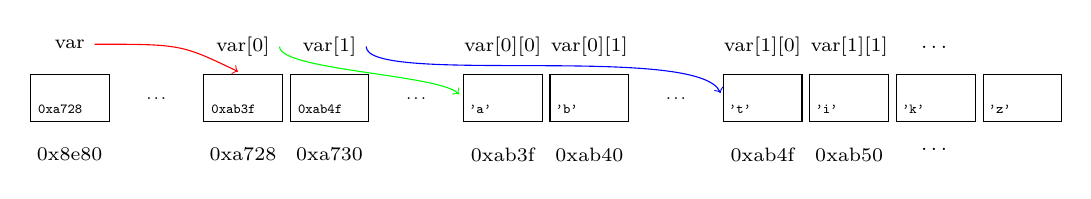
\begin{tikzpicture}
  [cell/.style={
		text width = 8mm,
		text height= 4mm,
		draw=black,
		inner sep=1mm
	},
    ld/.style={
		draw=blue,
		shorten >=2pt,
		->
	}]
  
  \node (c00) at ( 0  , 0) [cell] {\tiny\ttfamily 0xa728};
  \node (c01) at ( 1.1, 0)        {\tiny\ttfamily \ldots};
  \node (c02) at ( 2.2, 0) [cell] {\tiny\ttfamily 0xab3f};
  \node (c03) at ( 3.3, 0) [cell] {\tiny\ttfamily 0xab4f};
  \node (c04) at ( 4.4, 0)        {\tiny\ttfamily \ldots};
  \node (c05) at ( 5.5, 0) [cell] {\tiny\ttfamily 'a'};
  \node (c06) at ( 6.6, 0) [cell] {\tiny\ttfamily 'b'};
  \node (c07) at ( 7.7, 0)        {\tiny\ttfamily \ldots};
  \node (c08) at ( 8.8, 0) [cell] {\tiny\ttfamily 't'};
  \node (c09) at ( 9.9, 0) [cell] {\tiny\ttfamily 'i'};
  \node (c10) at (11.0, 0) [cell] {\tiny\ttfamily 'k'};
  \node (c11) at (12.1, 0) [cell] {\tiny\ttfamily 'z'};
  
  \node (avar0) [below=2mm of c00] {\scriptsize 0x8e80};
  \node (nvar0) [above=2mm of c00] {\scriptsize var};
  
  \node (avar1) [below=2mm of c02] {\scriptsize 0xa728};
  \node (nvar1) [above=1mm of c02] {\scriptsize var[0]};
  
  \node (avar2) [below=2mm of c03] {\scriptsize 0xa730};
  \node (nvar2) [above=1mm of c03] {\scriptsize var[1]};
  
  \node (avara) [below=2mm of c05] {\scriptsize 0xab3f};
  \node (nvara) [above=1mm of c05] {\scriptsize var[0][0]};
  
  \node (avarb) [below=2mm of c06] {\scriptsize 0xab40};
  \node (nvarb) [above=1mm of c06] {\scriptsize var[0][1]};
  
  \node (avarA) [below=2mm of c08] {\scriptsize 0xab4f};
  \node (nvarA) [above=1mm of c08] {\scriptsize var[1][0]};
  
  \node (avarA) [below=2mm of c09] {\scriptsize 0xab50};
  \node (nvarA) [above=1mm of c09] {\scriptsize var[1][1]};
  \node (vcont) [above=2mm of c10] {\scriptsize \ldots};
  \node (ncont) [below=2mm of c10] {\scriptsize \ldots};
  
  \draw [ld,draw=red  ] (nvar0.east) .. controls +( 1.1,  0  ) .. (c02.north);
  \draw [ld,draw=green] (nvar1.east) .. controls +( 0.0, -0.3) 
                                        and      +(-0.3, +0.3) .. (c05.west);
  \draw [ld           ] (nvar2.east) .. controls +( 0.0, -0.5) 
                                        and      +(-0.3, +0.7) .. (c08.west);
\end{tikzpicture}
\end{tcolorbox}
%
\end{frame}

% =========================================================================== %

\begin{frame}[fragile]{In Code}
%
\begin{codebox}[eindimensionale Repräsentation]
\begin{minted}[fontsize=\scriptsize]{text}
Datentyp * matrix = malloc(  Zeilen * Spalten * sizeof(Datentyp)  );

matrix[ID_Zeile * Spalten + ID_spalte] = Wert;

free(matrix);
\end{minted}
\end{codebox}
%
\begin{codebox}[mehrdimensionale Repräsentation]
\begin{minted}[fontsize=\scriptsize]{text}
Datentyp ** matrix          = malloc(  Zeilen  * sizeof( *matrix)  );
matrix[ID_Zeile]            = malloc(  Spalten * sizeof(**matrix)  );

matrix[ID_Zeile][ID_Spalte] = value;

free( matrix[ID_Zeile] );
free( matrix           );
\end{minted}
\end{codebox}
%
\end{frame}

% =========================================================================== %

\begin{frame}[fragile]
%
\tcbset{width=.495\linewidth, on line, height=7.2cm}
%
\begin{codebox}[Beispiel: 1D-Matrix-Repräsentation]
\begin{minted}[fontsize=\scriptsize, linenos]{c}
#include <stdio.h>
#include <stdlib.h>

int main() {
  int N, i, r, c, lineStart;
	
  printf("please enter: matix width: ");
  scanf("%d", &N);
  printf("\n");
	
  if (N < 1) {
    printf("illeagal value!\n");
    return -1;
  }
	
  int * matrix = malloc(
             N * N * sizeof(*matrix)
        );
\end{minted}
\end{codebox}
%
\begin{codebox}[...Fortsetzung]
\begin{minted}[fontsize=\scriptsize, linenos, firstnumber=last]{c}
  lineStart = N * N - N;
  for (i = 0; i < N * N; i++) {
    matrix[i] = lineStart + i + 1;
    if (i % N == N - 1) {
      lineStart -= 2 * N;
    }
  }
	
  for   (r = 0; r < N; r++) {
    for (c = 0; c < N; c++) {
      printf("%d\t", matrix[r * N + c]);
    }
    printf("\n");
  }

  free(matrix);
}
\end{minted}
\end{codebox}
%
\end{frame}

% =========================================================================== %

\begin{frame}[fragile]
%
\tcbset{width=.495\linewidth, on line, height=7.2cm}
%
\begin{codebox}[Beispiel: 2D-Matrix-Repräsentation]
\begin{minted}[fontsize=\scriptsize, linenos, firstnumber = 16]{c}
...
int ** matrix = malloc(
       N * sizeof(*matrix)
);
for (i = 0; i < N; i++) {
   matrix[i] = malloc(
                  N * sizeof(*matrix[i])
               );
}

lineStart = N * N - N;

for    (r = 0; r < N; r++) {
   for (c = 0; c < N; c++) {
      matrix[r][c] = lineStart + c + 1;
   }
   lineStart -= N;
}
\end{minted}
\end{codebox}
%
\begin{codebox}[...Fortsetzung]
\begin{minted}[fontsize=\scriptsize, linenos, firstnumber=last]{c}
for    (r = 0; r < N; r++) {
   for (c = 0; c < N; c++) {
      printf("%d\t", matrix[r][c]);
   }
   printf("\n");
}

for (i = 0; i < N; i++) {
   free(matrix[i]);
}
free(matrix);
\end{minted}
\end{codebox}
%
\end{frame}

% =========================================================================== %

\begin{frame}
%
\begin{hintbox}[Ein Index vs. mehrere Indizes -- welche Technik wann?]
In der Praxis: Fast immer \enquote{geplättete Listen} zu bevorzugen. Weniger Fehleranfällig, effizientere Code-Ausführung.\\
Vergleiche automatische Arrays: Compiler setzt diese intern als einfaches Array um.\\
Einziger Vorteil für Multi-Index-Listen: Spalten unterschiedlicher Länge können Speicherschonender umgesetzt werden. (Dann aber eine zusätzliche Liste der Spaltenlängen nötig.)
\end{hintbox}
%
\end{frame}

% =========================================================================== %

\begin{frame}{\emph{Heap} und \emph{Stack}}
%
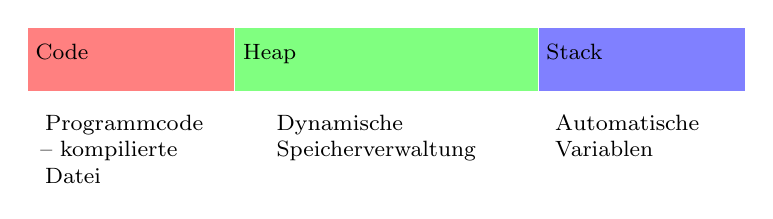
\begin{tikzpicture}
\footnotesize
\node (code) 
	[text height=3mm, text depth=3mm, text width=.2\linewidth, fill=red!50!white]
	{Code};
\node (heap) 
	[text height=3mm, text depth=3mm, text width=.3\linewidth, fill=green!50!white, right=0pt of code] 
	{Heap};
\node (stack) 
	[text height=3mm, text depth=3mm, text width=.2\linewidth, fill=blue!50!white,  right=0pt of heap] 
	{Stack};
	
\node (tcode) 
	[below=2mm of code, text width=.18\linewidth, font=\rightskip0pt plus 1fil]
	{Programmcode -- kompilierte Datei};
\node (theap) 
	[below=2mm of heap, text width=.23\linewidth, font=\rightskip0pt plus 1fil]
	{Dynamische Speicherverwaltung};
\node (tstack) 
	[below=2mm of stack,text width=.18\linewidth, font=\rightskip0pt plus 1fil]
	{Automatische Variablen};
\end{tikzpicture}
%
\hspace{10pt}
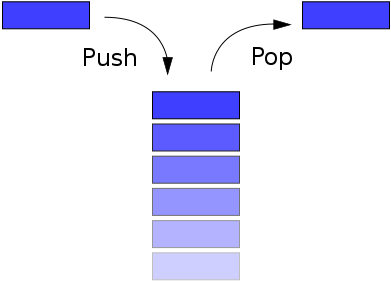
\includegraphics[width=.2\linewidth]{./gfx/Stack}
%
\begin{columns}[T]
\column{.46\linewidth}
\begin{itemize}
\item Einteilung Speicher in mehere Bereiche
\item Historisch gewachsen
\item Code-Segment -- nur Lese-Zugriffe vorgesehen
\end{itemize}
%
\column{.46\linewidth}
\begin{itemize}
\item Stack (\emph{Stapel}) -- klein, automatische Verwaltung vom OS; daher \emph{starre} Struktur
\item Heap (\emph{Halde, Haufen}) -- groß, Verwaltung durch ProgrammiererIn, freie Strukturgestaltung zur Laufzeit
\end{itemize}
\end{columns}
%
\end{frame}

% =========================================================================== %

\begin{frame}{Vergleich: Automatische und dynamische Arrays}
%
\rowcolors{1}{white}{chameleonblue2}
\newcolumntype{A}{>{\centering\arraybackslash} m{.21\linewidth}}
\newcolumntype{D}{>{\centering\arraybackslash} m{.35\linewidth}}
\newcolumntype{U}{>{\centering\arraybackslash} m{.70\linewidth}}
%
\begin{tabularx}
	{\linewidth}
	{A|D|D}
	
	\toprule
	
	& \textbf{automatische Arrays} & \textbf{dynamische Arrays} \tabcrlf

	Anlegen	
	& \texttt{datatype variable[count]}
	& über \texttt{malloc} oder \texttt{calloc}
	\\
	Zugriff
	& \multicolumn{2}{U}{über Pointer: \texttt{variable[index]}\newline oder \texttt{*(variable + index)}}
	\\
	Größe ändern
	& nicht möglich
	& über \texttt{realloc}
	\\
	Größe abfragen 
	& über \texttt{sizeof} (Größe des gesamten Arrays \emph{in Bytes})
	& nicht möglich -- Information beim Anlegen \enquote{aufbewahren}
	\\
	Größe eines Elements abfragen 
	& \multicolumn{2}{U}{\texttt{sizeof(*variable)}}
	\\
	Speicher Freigeben 
	& nicht nötig
	& über \texttt{free}	
	\\
	Multi-Index 
	& einfach
	& schwer
	\\
	Speicherort
	& im Stack
	& im Heap 
	\\
	
	\bottomrule
\end{tabularx}

%
\end{frame}
\end{document}